\documentclass[11pt, a4paper, twoside]{article}

% Version en 2024 Víctor Bettachini < vbettachini@unlam.edu.ar >

\usepackage[T1]{fontenc}
\usepackage[utf8]{inputenc}

% \usepackage[spanish, es-tabla]{babel}
% \def\spanishoptions{argentina} % Was macht dass?
% \usepackage{babelbib}
% \selectbiblanguage{spanish}
% \addto\shorthandsspanish{\spanishdeactivate{~<>}}

\usepackage{graphicx}
\graphicspath{{../figuresLaTeX/}}
% \usepackage{float}

\usepackage[arrowdel]{physics}
\newcommand{\pvec}[1]{\vec{#1}\mkern2mu\vphantom{#1}}
% \usepackage{units}
\usepackage[separate-uncertainty= true, multi-part-units= single, range-units= single, range-phrase= {~a~}, locale= FR]{siunitx}
\usepackage{isotope} % $\isotope[A][Z]{X}\to\isotope[A-4][Z-2]{Y}+\isotope[4][2]{\alpha}

\usepackage{tasks}
\usepackage[inline]{enumitem}
% \usepackage{enumerate}

\usepackage{hyperref}

% \usepackage{amsmath}
% \usepackage{amstext}
% \usepackage{amssymb}

\usepackage{tikz}
\usepackage{tikz-3dplot}
\usepackage{tikz-dimline}
\usetikzlibrary{calc}
% \usetikzlibrary{math}
\usetikzlibrary{arrows.meta}
\usetikzlibrary{snakes}
\usetikzlibrary{decorations}
\usetikzlibrary{decorations.pathmorphing}
\usetikzlibrary{patterns}

\usepackage[hmargin=1cm,vmargin=3cm, top= 0.75cm,nohead]{geometry}

\usepackage{lastpage}
\usepackage{fancyhdr}
\pagestyle{fancyplain}
\fancyhf{}
\setlength\headheight{28.7pt} 
\fancyhead[LE, LO]{\textbf{Computational Analytical Mechanics} }
% \fancyhead[LE, LO]{\textbf{Mecánica General} }
\fancyhead[RE, RO]{\href{https://ingenieria.unlam.edu.ar/}{$\vcenter{\hbox{\includegraphics[height=1cm]{ambos.pdf}}}$}}
\fancyfoot{\href{https://creativecommons.org/licenses/by-nc-sa/4.0/}{$\vcenter{\hbox{\includegraphics[height=0.4cm]{by-nc-sa_80x15.pdf}}}$} \href{https://ingenieria.unlam.edu.ar/}{DIIT - UNLaM}}
\fancyfoot[C]{ {\tiny Updated \today} }
\fancyfoot[RO, LE]{Page \thepage/\pageref{LastPage}}
\renewcommand{\headrulewidth}{0pt}
\renewcommand{\footrulewidth}{0pt}


\begin{document}
\begin{center}
  \textsc{\large Rigid body | Inertia tensors}
\end{center}

\begin{enumerate}
	\item
	\textbf{Carbon monoxide}\\
	Calculating the inertia tensor of a molecule requires knowing the distance between the atoms and their masses.

	The distance, or bodn length, can be found at the \href{https://cccbdb.nist.gov/exp1x.asp}{Computational Chemistry Comparison and Benchmark DataBase} of the National Institute of Standards and Technology, NIST, U.S.A.
	Querying about the chemical formula, \emph{CO} in this case, we can find the distances, or the positions in a cartesian frame of reference, expressed in \si{angstrom}, equivalent to \SI{1e-10}{\metre}.

	The mass for each chemical element is expressed in unified atomic mass units, \si{\atomicmassunit}, in the \href{https://iupac.org/what-we-do/periodic-table-of-elements/}{periodic table} published by the International Union of Pure and Applied Chemistry, IUPAC. This is the mass expressed in grams of one mole of atoms with the proportion of isotopes found in nature. To obtain the mass in grams of just one atom, simply divide by the number of atoms in this mole, Avogadro's constant, \(N_A = \SI{6.022e23}{\per\mole}\).

	Express the inertia tensor in SI units (\si{\kilogram \squared \metre}).
	Result:\\
	\[
		\overline{\overline{I}} = \left[\begin{matrix}0 & 0 & 0\\0 & 1.45 \cdot 10^{-46} & 0\\0 & 0 & 1.45 \cdot 10^{-46}\end{matrix}\right]
	\]



	\item 
	\begin{minipage}[t][3cm]{0.73\textwidth}
	\textbf{Water}\\
		Express the inertia tensor in SI units.
		Result:\\
		\[
			\overline{\overline{I}} = \left[\begin{matrix}1.02 \cdot 10^{-47} & 0 & 0\\0 & 1.92 \cdot 10^{-47} & 0\\0 & 0 & 2.95 \cdot 10^{-47}\end{matrix}\right]
		\]
	\end{minipage}
	\begin{minipage}[c][0.5cm][t]{0.2\textwidth}
		\includegraphics[width=\textwidth]{figures/moleculaH2O}
	\end{minipage}

	

	\item 
	\begin{minipage}[t][3cm]{0.73\textwidth}
	\textbf{Dichloromethane}\\
	The chemical formula for this molecule is \isotope{CH_2Cl_2}. Express the inertia tensor in SI units.
		Result:\\
		\[
			\overline{\overline{I}} = \left[\begin{matrix}2.69 \cdot 10^{-46} & 0 & 0\\0 & 2.56 \cdot 10^{-45} & 0\\0 & 0 & 1.04 \cdot 10^{-36}\end{matrix}\right]
		\]
	\end{minipage}
	\begin{minipage}[c][0.5cm][t]{0.2\textwidth}
		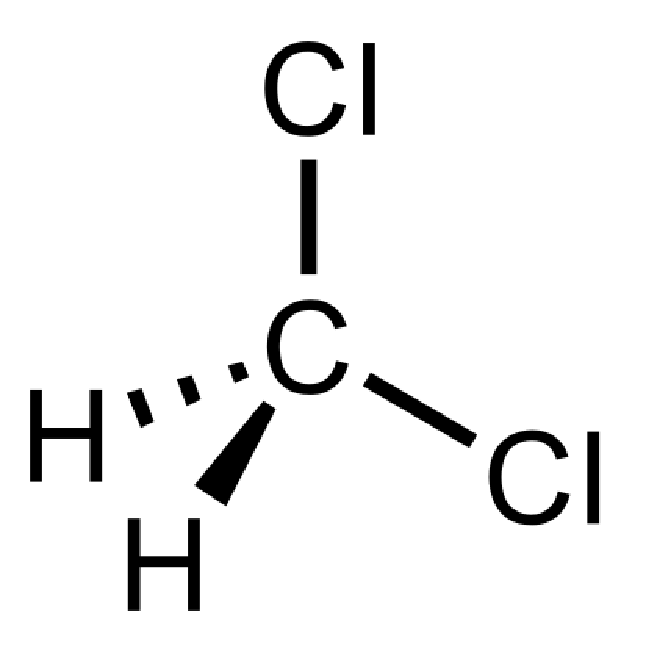
\includegraphics[width=\textwidth]{figures/Dichloromethane_molecular_structure}
	\end{minipage}



	\item 
	\begin{minipage}[t][6cm]{0.65\textwidth}
		\textbf{Unbalanced torsion pendulum}\\
		The figure shows a system at \(t = 0 \) with weights at the ends of two arms.
		The vertical rod rotates without friction at a constant angular velocity $\Omega$ with respect to the inertial frame of reference $O_{xyz}$. The rod and the arms have negligible masses, compared to the mass \(m\) of each weight.
		Calculate: 
		\begin{tasks} 
			\task the inertia tensor with respect to A as a function of time \(\overline{\overline{I}}_A(t)\)\\
			\task the angular momentum $\vec{L}_A (t) = \overline{\overline{I}}_A (t) \vec{\Omega}$ and torque $\vec{\tau} (t) = \dot{\vec{L}} (t)$.
		\end{tasks}
	\end{minipage}
	\begin{minipage}[c][0cm][t]{0.3\textwidth}
		\includegraphics[width=\textwidth]{figures/o-021}
	\end{minipage}
	Results:\\
			\[
				\scalebox{0.9}{$
				\overline{\overline{I}}_A = \left[\begin{matrix}\ell^{2} m \left(- \cos^{2}{\left(\phi \right)} \cos^{2}{\left(\Omega t \right)} - \cos^{2}{\left(\Omega t \right)} + 2\right) & - \ell^{2} m \left(\cos^{2}{\left(\phi \right)} + 1\right) \sin{\left(\Omega t \right)} \cos{\left(\Omega t \right)} & \frac{\ell^{2} m \left(\sin{\left(\Omega t - 2 \phi \right)} - \sin{\left(\Omega t + 2 \phi \right)}\right)}{4}\\- \ell^{2} m \left(\cos^{2}{\left(\phi \right)} + 1\right) \sin{\left(\Omega t \right)} \cos{\left(\Omega t \right)} & \ell^{2} m \left(\sin^{2}{\left(\phi \right)} \sin^{2}{\left(\Omega t \right)} - 2 \sin^{2}{\left(\Omega t \right)} + 2\right) & - \frac{\ell^{2} m \left(\cos{\left(\Omega t - 2 \phi \right)} - \cos{\left(\Omega t + 2 \phi \right)}\right)}{4}\\\frac{\ell^{2} m \left(\sin{\left(\Omega t - 2 \phi \right)} - \sin{\left(\Omega t + 2 \phi \right)}\right)}{4} & - \frac{\ell^{2} m \left(\cos{\left(\Omega t - 2 \phi \right)} - \cos{\left(\Omega t + 2 \phi \right)}\right)}{4} & \ell^{2} m \left(\cos^{2}{\left(\phi \right)} + 1\right)\end{matrix}\right]
				$}
				\] 
			\[
				\vec{L}_A = \left[\begin{matrix}\frac{\Omega \ell^{2} m \left(\sin{\left(\Omega t - 2 \phi \right)} - \sin{\left(\Omega t + 2 \phi \right)}\right)}{4}\\- \frac{\Omega \ell^{2} m \left(\cos{\left(\Omega t - 2 \phi \right)} - \cos{\left(\Omega t + 2 \phi \right)}\right)}{4}\\\Omega \ell^{2} m \left(\cos^{2}{\left(\phi \right)} + 1\right)\end{matrix}\right]
			\qquad
				\vec{\tau}_A = \left[\begin{matrix}\frac{\Omega^{2} \ell^{2} m \left(\cos{\left(\Omega t - 2 \phi \right)} - \cos{\left(\Omega t + 2 \phi \right)}\right)}{4}\\\frac{\Omega^{2} \ell^{2} m \left(\sin{\left(\Omega t - 2 \phi \right)} - \sin{\left(\Omega t + 2 \phi \right)}\right)}{4}\\0\end{matrix}\right]
			\]


	\end{enumerate}

\end{document}
